%%%%%%%%%%%%%%%%%%%%%%%%%%%%%%%%%%%%%%%%%%%%%%%%%%%%%%%%%%%%%%%%%%
\begin{frame}{Another view of a sequence}
    \begin{center}
      \begin{displaymath}
          \begin{array}{lcccccccc}
            \seq{s}=&[ &\cgc&\cga&\cgt&\cgt&\cgg&\cgt
                        &]\\
            &&\downarrow &\downarrow &\downarrow &\downarrow &\downarrow &\downarrow \\
            \textrm{Look-up}&&\wemb &\wemb &\wemb &\wemb &\wemb &\wemb  \\
               &&\wvector_{\cgc}&\wvector_{\cga}&\wvector_{\cgt}&\wvector_{\cgt}&\wvector_{\cgg}&\wvector_{\cgt} \\
          \end{array}
        \end{displaymath}
        {\huge $\downarrow$} \\
        \tikz{\draw[step=0.5,black,thin] (0,0) grid (3,2);}
    \end{center}
\end{frame}



%%%%%%%%%%%%%%%%%%%%%%%%%%%%%%%%%%%%%%%%%%%%%
\begin{frame}
  \frametitle{Inspiration}
  \begin{block}{Convolutional Neural Networks for Sentence
      Classification}
    \begin{itemize}
    \item A short paper of 2014~\cite{Kim14Convolution}
    \item A simple and SOTA paper on text classification
    \end{itemize}
  \end{block}
  \begin{block}{Highlights}
    \begin{columns}
      \column{0.3\textwidth}{
        \begin{center}
          $\x$\\[1ex]
          {\huge $\downarrow$} \\[1ex]
          \tikz{\draw[step=0.5,black,thin] (0,0) grid (3,2);}
      \end{center}
    }
    %%%%
    \column{0.7\textwidth}{%
      \begin{itemize}
      \item This input matrix is a sequence of vectors 
      \item We can extract features with convolution filters
      \item The filters and the embeddings are parameters \\(to be learnt)
      \end{itemize}
    }
    \end{columns}
  \end{block}
  Application to DNA classification in~\cite{Xu17Enhancer,Cohn18Enhancer}
\end{frame}


%%%%%%%%%%%%%%%%%%%%%%%%%%%%%%%%%%%%%%%%%%%%%%%%%%%%%%%%%%%%%%%%%%
% In pytorch the indices are :
% batch, channel, data-point
% The data point for a 1D input is (t,d)
% For an image it is (x,y)
\begin{frame}{Convolution 1D}
  \framesubtitle{Extract a frame, or a window, and apply a ``filter''}
  \begin{columns}
    \column{0.6\textwidth}
    %%% the input : a matrix + window
    \begin{center}
    The input sequence of  $L=6$ \\vectors in $\real^{\nfeats}$,  $\nfeats=4$ \\[1ex]
    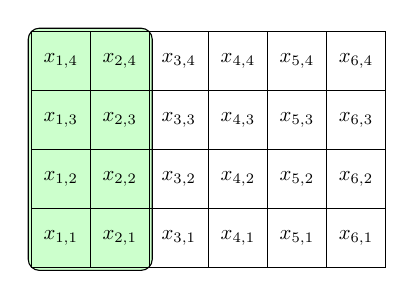
\begin{tikzpicture}[scale=0.75,every node/.style={scale=0.75}]
      % the window
      % offset for x and y of .5 + a bit more 
      \draw[fill=green!20,rounded corners] (0.45,0.45) rectangle (2.55,4.55); % green 
      %% the grid 
      \foreach \l in {1,2,...,4}
      \foreach \c in {1,2,...,6}
      {
        \draw (\c,\l) +(-.5,-.5) rectangle ++(.5,.5);
        \draw (\c,\l) node{$x_{\c,\l}$};
      }
    \end{tikzpicture}
  \end{center}
    \column{0.6\textwidth}
    \begin{center}
    The filter:\\kernel size of $ks=2$\\[1ex]
    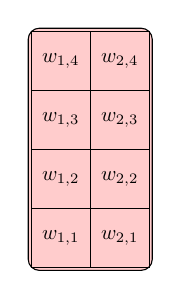
\begin{tikzpicture}[scale=0.75,every node/.style={scale=0.75}]
      % the window
      % offset for x and y of .5 + a bit more 
      \draw[fill=red!20,rounded corners] (0.45,0.45) rectangle (2.55,4.55); % green 
      
      %% the grid 
      \foreach \l in {1,2,...,4}
      \foreach \c in {1,2}
      {
        \draw (\c,\l) +(-.5,-.5) rectangle ++(.5,.5);
        \draw (\c,\l) node{$w_{\c,\l}$};
      }
    \end{tikzpicture}
  \end{center}
\end{columns}
\begin{block}{The output value (output channel)}
  $$
  \textrm{At time }t = 1,\ {\color{red!70!black} h_1} = \sum_{i,j} {\color{red!70!black}w_{i,j}}\times  {\color{green!70!black}x_{i,j}}
  $$
\end{block}
\end{frame}


%%%%%%%%%%%%%%%%%%%%%%%%%%%%%%%%%%%%%%%%%%%%%%%%%%%%%%%%%%%%%%%%%%%%%%%%%%%
\newcommand{\xs}{4}
\newcommand{\ys}{-4}
\begin{frame}{Convolution 1D: sliding along one dimension}
  \framesubtitle{Stride, or a sliding window}
  The input  is a matrix $(L=6,d=4)$, one filter of kernel size $=2$:~\\[1ex]
  \begin{block}{With a stride $= 1$}
    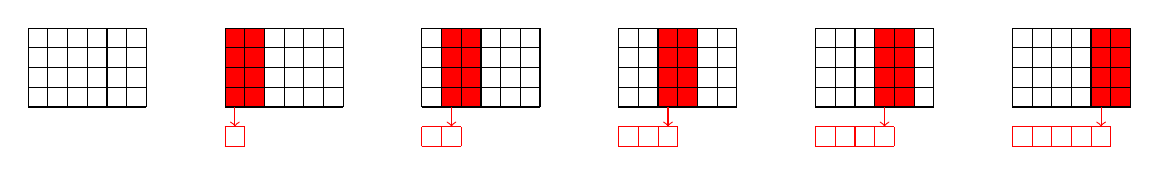
\begin{tikzpicture}[scale=0.5]
      %% the grid 
      \draw[step=0.5,black,thin] (0,0) grid (3,2);
      %%%%%%% 1 
      \draw[fill=red] (0+\xs,0) rectangle (1+\xs,2); % red 
      \draw[step=0.5,black,thin] (0+\xs,0) grid (3+\xs,2); % grid
      \draw[step=0.5,red] (-0.01+\xs,-0.5) grid (0.5+\xs,-1);    % grid res
      % arrow
      \draw[->,red]   (0.25+\xs,0) --  (0.25+\xs,-0.5);
      %%%%%%% 2 
      \draw[fill=red] (0.5+2*\xs,0) rectangle (1.5+2*\xs,2); % red 
      \draw[step=0.5,black,thin] (-0.01+2*\xs,0) grid (3+2*\xs,2); % grid
      \draw[step=0.5,red] (-0.01+2*\xs,-0.5) grid (1+2*\xs,-1);    % grid res
      % arrow
      \draw[->,red]   (0.75+2*\xs,0) --  (0.75+2*\xs,-0.5);

      %%%%%%% 3 
      \draw[fill=red] (0.99+3*\xs,0) rectangle (2+3*\xs,2); % red 
      \draw[step=0.5,black,thin] (-0.01+3*\xs,0) grid (3+3*\xs,2); % grid
      \draw[step=0.5,red] (-0.01+3*\xs,-0.5) grid (1.5+3*\xs,-1);    % grid res
      % arrow
      \draw[->,red]   (1.25+3*\xs,0) --  (1.25+3*\xs,-0.5);

      %%%%%%% 4
      \draw[fill=red] (1.49+4*\xs,0) rectangle (2.5+4*\xs,2); % red 
      \draw[step=0.5,black,thin] (-0.01+4*\xs,0) grid (3+4*\xs,2); % grid
      \draw[step=0.5,red] (-0.01+4*\xs,-0.5) grid (2+4*\xs,-1);    % grid res
      % arrow
      \draw[->,red]   (1.75+4*\xs,0) --  (1.75+4*\xs,-0.5);

      %%%%%%% 5 
      \draw[fill=red] (1.99+5*\xs,0) rectangle (3+5*\xs,2); % red 
      \draw[step=0.5,black,thin] (-0.01+5*\xs,0) grid (3+5*\xs,2); % grid
      \draw[step=0.5,red] (-0.01+5*\xs,-0.5) grid (2.5+5*\xs,-1);    % grid res
      % arrow
      \draw[->,red]   (2.25+5*\xs,0) --  (2.25+5*\xs,-0.5);
    \end{tikzpicture}
  \end{block}
  \begin{block}{With a stride = 2}
    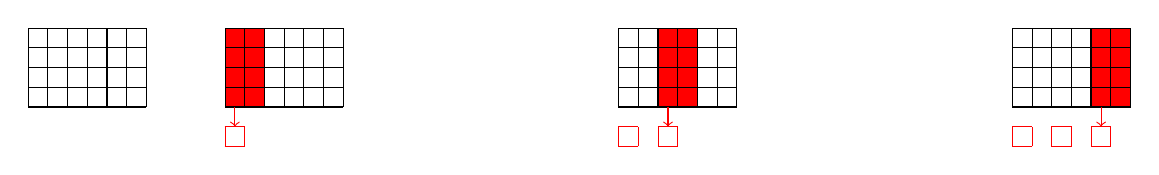
\begin{tikzpicture}[scale=0.5]
      %% the grid 
      \draw[step=0.5,black,thin] (0,0) grid (3,2);
      %%%%%%% 1 
      \draw[fill=red] (0+\xs,0) rectangle (1+\xs,2); % red 
      \draw[step=0.5,black,thin] (0+\xs,0) grid (3+\xs,2); % grid
      \draw[step=0.5,red] (-0.01+\xs,-0.5) grid (0.5+\xs,-1);    % grid res
      \draw[->,red]   (0.25+\xs,0) --  (0.25+\xs,-0.5);       % arrow

      %%%%%%% 3 
      \draw[fill=red] (0.99+3*\xs,0) rectangle (2+3*\xs,2); % red 
      \draw[step=0.5,black,thin] (-0.01+3*\xs,0) grid (3+3*\xs,2); % grid
      \draw[step=0.5,red] (-0.01+3*\xs,-0.5) grid (0.5+3*\xs,-1);    % grid res
      \draw[step=0.5,red] (-0.01+3*\xs+1,-0.5) grid (1.5+3*\xs,-1);    % grid res
      % arrow
      \draw[->,red]   (1.25+3*\xs,0) --  (1.25+3*\xs,-0.5);
      %%%%%%% 5 
      \draw[fill=red] (1.99+5*\xs,0) rectangle (3+5*\xs,2); % red 
      \draw[step=0.5,black,thin] (-0.01+5*\xs,0) grid (3+5*\xs,2); % grid
      \draw[step=0.5,red] (-0.01+5*\xs,-0.5) grid (0.5+5*\xs,-1);    % grid res
      \draw[step=0.5,red] (-0.01+5*\xs+1,-0.5) grid (1.5+5*\xs,-1);    % grid res
      \draw[step=0.5,red] (-0.01+5*\xs+2,-0.5) grid (2.5+5*\xs,-1);    % grid res
      % arrow
      \draw[->,red]   (2.25+5*\xs,0) --  (2.25+5*\xs,-0.5);
    \end{tikzpicture}
  \end{block}
\end{frame}


%%%%%%%%%%%%%%%%%%%%%%%%%%%%%%%%%%%%%%%%%%%%%%%%%%%%%%%%%%%%%%%%%%%%%%%%%%%%%%%%%%%%%%%% 
\begin{frame}{Convolution 1D}
  \framesubtitle{With 2 output channels}
  \begin{columns}
    \column{0.6\textwidth}
    %%% the input : a matrix + window
    \begin{center}
      $L=6$,  $\nfeats=4$ \\[1ex]
      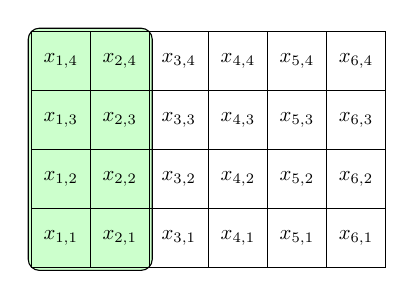
\begin{tikzpicture}[scale=0.75,every node/.style={scale=0.75}]
        % the window
        % offset for x and y of .5 + a bit more 
        \draw[fill=green!20,rounded corners] (0.45,0.45) rectangle (2.55,4.55); % green 
        %% the grid 
        \foreach \l in {1,2,...,4}
        \foreach \c in {1,2,...,6}
        {
          \draw (\c,\l) +(-.5,-.5) rectangle ++(.5,.5);
          \draw (\c,\l) node{$x_{\c,\l}$};
        }
      \end{tikzpicture}
    \end{center}
    \column{0.4\textwidth}
    \begin{center}
      Filters:kernel size of $ks=2$\\[1ex]
      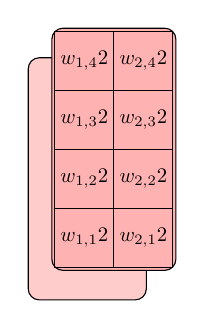
\begin{tikzpicture}[scale=0.75,every node/.style={scale=0.75}]
        % the window
        % offset for x and y of .5 + a bit more 
        \draw[fill=red!20,rounded corners] (0.05,-0.05) rectangle (2.05,4.05); % first 
        \draw[fill=red!30,rounded corners] (0.45,0.45) rectangle (2.55,4.55); 
        %% the grid 
        \foreach \l in {1,2,...,4}
        \foreach \c in {1,2}
        {
          \draw (\c,\l) +(-.5,-.5) rectangle ++(.5,.5);
          \draw (\c,\l) node{$w_{\c,\l}\lid{2}$};
        }
      \end{tikzpicture}
    \end{center}
  \end{columns}
  \begin{block}{The output value (output channel)}
    \begin{align*}
      {\color{red!70!black} h_{1,1}} &= \sum_{i,j} {\color{red!70!black}w_{i,j}\lid{1}}\times  {\color{green!70!black}x_{i,j}} \\
      {\color{red!70!black} h_{2,1}} &= \sum_{i,j} {\color{red!70!black}w_{i,j}\lid{2}}\times  {\color{green!70!black}x_{i,j}} 
    \end{align*}
  \end{block}
\end{frame}



%%%%%%%%%%%%%%%%%%%%%%%%%%%%%%%%%%%%%%%%%%%%%%%%%%%%%%%%%%%%%%%%%%%%%%%%%%%%%%%%%%%%%%%% 
\begin{frame}{Another wiew for two output channels}
  \begin{columns}
    \column{0.5\textwidth}
    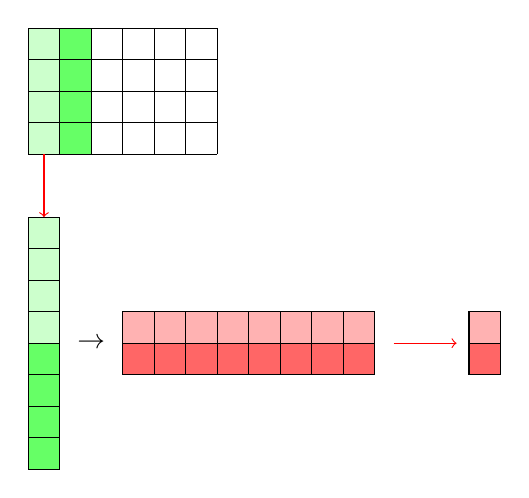
\begin{tikzpicture}[scale=0.8]
      %%%%%%% the sentence as a matrix
    \draw[fill=green!20] (0,0) rectangle (0.5,2); % red 
    \draw[fill=green!60] (0.5,0) rectangle (1,2); % red 
    \draw[step=0.5,black,thin] (0,0) grid (3,2); % grid
    %%%%% window extract 
    \draw[fill=green!60] (0,-1+\ys) rectangle (0.5,1+\ys); % red
    \draw[fill=green!20] (0,1+\ys) rectangle (0.5,3+\ys); % red
    \draw[step=0.5,black,thin] (0,-1+\ys) grid (0.5,3+\ys); % grid
    %%%  
    \draw[->,red] (0.25,0) -- (0.25,-1); % arrow
    %%% Filter 
    \node (times) at (1,1+\ys) {$\rightarrow$};
    \draw[fill=red!60] (1.49,0.5+\ys) rectangle (1.5+4,1+\ys); % colors
    \draw[fill=red!30] (1.49,1+\ys) rectangle (1.5+4,1.5+\ys); % colors 
    \draw[step=0.5,black] (1.49,0.5+\ys) grid (1.5+4,1.5+\ys); % grid
    \node (times) at (4,-0.5+\ys) {$\W$};
    %%%
    \draw[->,red] (5.8,1+\ys) -- (6.8,1+\ys); % arrow
    \draw[fill=red!60] (7-0.01,0.5+\ys) rectangle (7.5,1+\ys); % grid
    \draw[fill=red!30] (7-0.01,1+\ys) rectangle (7.5,1.5+\ys); % grid
    \draw[step=0.5,thin] (7-0.01,0.5+\ys) grid (7.5,1.5+\ys); % grid
  \end{tikzpicture}
  \column{0.5\textwidth}
  \begin{itemize}
  \item {\color{red!30!black} Two filters } applied to the same {\color{green!30!black} frame (or window)}
  \item Each filter generates one feature 
  \item[$\rightarrow$]  a vector of two values, two features $( h_{1,1},  h_{2,1})$
  \item $ h_{c,t}$ is the feature extracted for the channel $c$ at time $t$. 
  \item $\W$ gathers the parameters of the filters in one matrix
  \item The parameters $\W$ are learnt
  \end{itemize}
\end{columns}

\end{frame}



%%%%%%%%%%%%%%%%%%%%%%%%%%%%%%%%%%%%%%%%%%%%%%%%%%%%%%%%%%%%%%%%%%%%%%%%%%%%%%%%%%%%%%%% 
\begin{frame}
  \frametitle{1D-convolution and pooling}
  The input text is a matrix $(L=6,d=4,od=2)$ after the embedding step:~\\[1ex]
  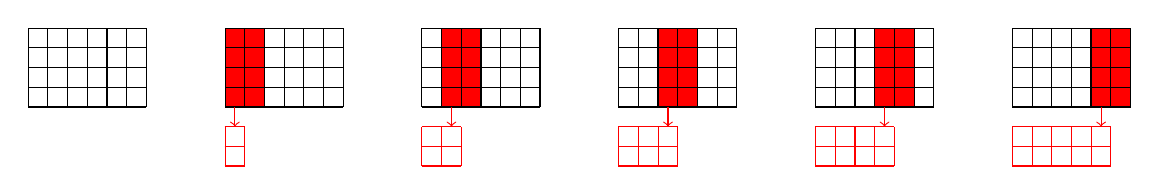
\begin{tikzpicture}[scale=0.5]
    %% the grid 
    \draw[step=0.5,black,thin] (0,0) grid (3,2);
  %%%%%%% 1 
    \draw[fill=red] (0+\xs,0) rectangle (1+\xs,2); % red 
    \draw[step=0.5,black,thin] (0+\xs,0) grid (3+\xs,2); % grid
    \draw[step=0.5,red] (-0.01+\xs,-0.5) grid (0.5+\xs,-1.5);    % grid res
    % arrow
    \draw[->,red]   (0.25+\xs,0) --  (0.25+\xs,-0.5);
  %%%%%%% 2 
    \draw[fill=red] (0.5+2*\xs,0) rectangle (1.5+2*\xs,2); % red 
    \draw[step=0.5,black,thin] (-0.01+2*\xs,0) grid (3+2*\xs,2); % grid
    %grid res
    \draw[step=0.5,red] (-0.01+2*\xs,-0.5) grid (1+2*\xs,-1.5);    % grid res
    % arrow
    \draw[->,red]   (0.75+2*\xs,0) --  (0.75+2*\xs,-0.5);

  %%%%%%% 3 
    \draw[fill=red] (0.99+3*\xs,0) rectangle (2+3*\xs,2); % red 
    \draw[step=0.5,black,thin] (-0.01+3*\xs,0) grid (3+3*\xs,2); % grid
    \draw[step=0.5,red] (-0.01+3*\xs,-0.5) grid (1.5+3*\xs,-1.5);    % grid res
    % arrow
    \draw[->,red]   (1.25+3*\xs,0) --  (1.25+3*\xs,-0.5);

  %%%%%%% 4
    \draw[fill=red] (1.49+4*\xs,0) rectangle (2.5+4*\xs,2); % red 
    \draw[step=0.5,black,thin] (-0.01+4*\xs,0) grid (3+4*\xs,2); % grid
    \draw[step=0.5,red] (-0.01+4*\xs,-0.5) grid (2+4*\xs,-1.5);    % grid res
    % arrow
    \draw[->,red]   (1.75+4*\xs,0) --  (1.75+4*\xs,-0.5);

  %%%%%%% 5 
    \draw[fill=red] (1.99+5*\xs,0) rectangle (3+5*\xs,2); % red 
    \draw[step=0.5,black,thin] (-0.01+5*\xs,0) grid (3+5*\xs,2); % grid
    \draw[step=0.5,red] (-0.01+5*\xs,-0.5) grid (2.5+5*\xs,-1.5);    % grid res
    % arrow
    \draw[->,red]   (2.25+5*\xs,0) --  (2.25+5*\xs,-0.5);

  \end{tikzpicture}\\[1ex]\vfill
  %%
  \begin{itemize}
  \item The transformation:  a matrix of size $(od, ws\times d)=(2, 8)$
  \item $ws$: window size
  \item $od$ is sometime called the number of featuremap. 
  \end{itemize}
  \begin{block}{Max-pooling over-time}
  \begin{center}
    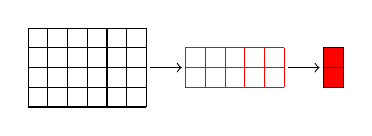
\begin{tikzpicture}[scale=0.5]
      %% the grid
      \draw[step=0.5,black,thin] (0,0) grid (3,2);
      \draw[->] (3.1,1)-- (3.9,1);
      \draw[step=0.5,red,thin] (3.99,0.5) grid (6.5,1.5);
      \draw[->] (6.6,1)-- (7.4,1);
      
      %%%%%%% final
      \draw[fill=red] (7.5,0.5) rectangle  (8,1.5); 
      \draw[step=0.5,black] (7.5,0.5) grid (8,1.5); % grid res
    \end{tikzpicture}
  \end{center}
\end{block}

\end{frame}



%%%%%%%%%%%%%%%%%%%%%%%%%%%%%%%%%%%%%%%%%%%%%%%%%%%%%%%%%%%%%%%%%%%%%%%%%%%%%%%%%%%%%%%% 
\renewcommand{\xs}{5}
\begin{frame}
  \frametitle{More Convolutions}
  \begin{center}
  The window size can vary: \\[3ex]
  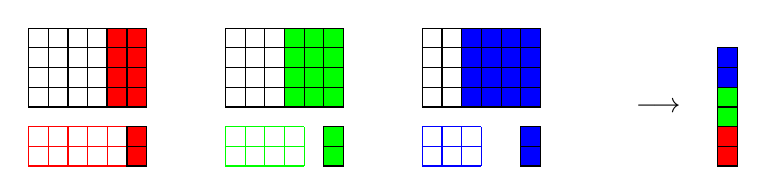
\begin{tikzpicture}[scale=0.5]
    %%%%%  for 2 
    \draw[fill=red] (1.99+0*\xs,0) rectangle (3+0*\xs,2); % red 
    \draw[step=0.5,black,thin] (-0.01+0*\xs,0) grid (3+0*\xs,2); % grid
    \draw[step=0.5,red] (-0.01+0*\xs,-0.5) grid (2.5+0*\xs,-1.5);    % grid res
    \draw[fill=red] (2.5-0.01+0*\xs,-0.5) rectangle (3+0*\xs,-1.5);    % polling
    \draw[step=0.5,black] (2.5-0.01+0*\xs,-0.5) grid (3+0*\xs,-1.5);    % pooling

    %% the grid for 3 
    \draw[fill=green] (1.5+1*\xs,0) rectangle (3+1*\xs,2); % green
    \draw[step=0.5,black,thin] (0-0.01+1*\xs,0) grid (3+1*\xs,2);
    \draw[step=0.5,green] (-0.01+1*\xs,-0.5) grid (2+1*\xs,-1.5);    % grid res
    \draw[fill=green] (2.5-0.01+1*\xs,-0.5) rectangle (3+1*\xs,-1.5);    % polling
    \draw[step=0.5,black] (2.5-0.01+1*\xs,-0.5) grid (3+1*\xs,-1.5);    % pooling

    %% the grid for 4
    \draw[fill=blue] (1+2*\xs,0) rectangle (3+2*\xs,2); % blue
    \draw[step=0.5,black,thin] (0-0.01+2*\xs,0) grid (3+2*\xs,2);
    \draw[step=0.5,blue] (-0.01+2*\xs,-0.5) grid (1.5+2*\xs,-1.5);    % grid res
    \draw[fill=blue] (2.5-0.01+2*\xs,-0.5) rectangle (3+2*\xs,-1.5);    % polling
    \draw[step=0.5,black] (2.5-0.01+2*\xs,-0.5) grid (3+2*\xs,-1.5);    % pooling
    %%%
    \node (fuu) at  (1-0.01+3*\xs,0) {$\longrightarrow$};    % polling 2
    %%% stacked results of the pooling 
    \draw[fill=red] (2.5-0.01+3*\xs,-0.5) rectangle (3+3*\xs,-1.5);    % polling 2
    \draw[step=0.5,black] (2.5-0.01+3*\xs,-0.5) grid (3+3*\xs,-1.5);    % pooling 2
    \draw[fill=green] (2.5-0.01+3*\xs,-0.5) rectangle (3+3*\xs,0.5);    % polling 3
    \draw[step=0.5,black] (2.5-0.01+3*\xs,-0.5) grid (3+3*\xs,0.5);    % pooling 3 
    \draw[fill=blue] (2.5-0.01+3*\xs,0.5) rectangle (3+3*\xs,1.5);    % polling 4
    \draw[step=0.5,black] (2.5-0.01+3*\xs,0.5) grid (3+3*\xs,1.5);    % pooling 4
  \end{tikzpicture}\\[3ex]
  And they can be combined (concatenation). 
\end{center}
\end{frame}

\begin{frame}
  \frametitle{Convolutional Neural Networks for Sentence
    Classification}
  \begin{itemize}
  \item Window (kernel) sizes : 3, 4, 5 with 100 feature maps for each
  \item Static/non-static/random/multi-channel word embeddings
  \item Auxiliary data for word embeddings:~w2v trained on 100 billion words from
    Google News ($dim=300$) 
  \item dropout on the penultimate layer (after
    the max-pooling)
  \item Relu and early stopping
  \end{itemize}
\end{frame}


\begin{frame}{Pooling}
  How to compress information along one dimension (e.g time) ? \\
  $\rightarrow$ Pooling 
  
  \begin{itemize}
  \item Max pooling: most common
  \item Average  pooling: like the sum
  \item k-Max pooling
  \end{itemize}

\end{frame}


\begin{frame}{An overview of sequence convolution}
  \begin{itemize}
  \item The CNN layer's responsibility is to extract meaningful
    sub-structures that are useful for the overall prediction task at
    hand. 
  \item A convolutional neural network is designed to identify
    indicative local predictors in a large structure, 
  \item and to combine them to produce a fixed size vector representation of the
    structure, 
  \item capturing the local aspects that are most informative
    for the prediction task at hand. 
  \item In the NLP case the convolutional architecture will identify
    $n$-grams that are predictive for the task at hand, without the need
    to pre-specify an embedding vector for each possible $n$-gram.
  \end{itemize}
\begin{flushright}
  Y. Goldberg in \cite{Goldberg15Primer}
\end{flushright}
\end{frame}




\begin{frame}{Sentence classification}
  \begin{center}
    \includegraphics[width=0.7\textwidth]{../figs/conv_sentence}    
  \end{center}
  From~\cite{Kim14Convolution}
\end{frame}

\begin{frame}{Enhancer detection in DNA sequence}
  \begin{center}
    \includegraphics[width=0.7\textwidth]{../figs/conv_dna}    
  \end{center}
  From~\cite{Xu17Enhancer}
\end{frame}




